\documentclass[11pt,a4paper]{report}
\usepackage[textwidth=37em,vmargin=30mm]{geometry}
\usepackage{calc,xunicode,amsmath,amssymb,paralist,enumitem,tabu,booktabs,datetime2,xeCJK,xeCJKfntef,listings}
\usepackage{tocloft,fancyhdr,tcolorbox,xcolor,graphicx,eso-pic,xltxtra,xelatexemoji}

\newcommand{\envyear}[0]{2025}
\newcommand{\envdatestr}[0]{2025-07-08}
\newcommand{\envfinaldir}[0]{webdb/2025/20250708/final}

\usepackage[hidelinks]{hyperref}
\hypersetup{
    colorlinks=false,
    pdfpagemode=FullScreen,
    pdftitle={Web Digest - \envdatestr}
}

\setlength{\cftbeforechapskip}{10pt}
\renewcommand{\cftchapfont}{\rmfamily\bfseries\large\raggedright}
\setlength{\cftbeforesecskip}{2pt}
\renewcommand{\cftsecfont}{\sffamily\small\raggedright}

\setdefaultleftmargin{2em}{2em}{1em}{1em}{1em}{1em}

\usepackage{xeCJK,xeCJKfntef}
\xeCJKsetup{PunctStyle=plain,RubberPunctSkip=false,CJKglue=\strut\hskip 0pt plus 0.1em minus 0.05em,CJKecglue=\strut\hskip 0.22em plus 0.2em}
\XeTeXlinebreaklocale "zh"
\XeTeXlinebreakskip = 0pt


\setmainfont{Brygada 1918}
\setromanfont{Brygada 1918}
\setsansfont{IBM Plex Sans}
\setmonofont{JetBrains Mono NL}
\setCJKmainfont{Noto Serif CJK SC}
\setCJKromanfont{Noto Serif CJK SC}
\setCJKsansfont{Noto Sans CJK SC}
\setCJKmonofont{Noto Sans CJK SC}

\setlength{\parindent}{0pt}
\setlength{\parskip}{8pt}
\linespread{1.15}

\lstset{
	basicstyle=\ttfamily\footnotesize,
	numbersep=5pt,
	backgroundcolor=\color{black!5},
	showspaces=false,
	showstringspaces=false,
	showtabs=false,
	tabsize=2,
	captionpos=b,
	breaklines=true,
	breakatwhitespace=true,
	breakautoindent=true,
	linewidth=\textwidth
}






\newcommand{\coverpic}[2]{
    % argv: itemurl, authorname
    Cover photo by #2~~(\href{#1}{#1})
}
\newcommand{\makeheader}[0]{
    \begin{titlepage}
        % \newgeometry{hmargin=15mm,tmargin=21mm,bmargin=12mm}
        \begin{center}
            
            \rmfamily\scshape
            \fontspec{BaskervilleF}
            \fontspec{Old Standard}
            \fontsize{59pt}{70pt}\selectfont
            WEB\hfill DIGEST
            
            \vfill
            % \vskip 30pt
            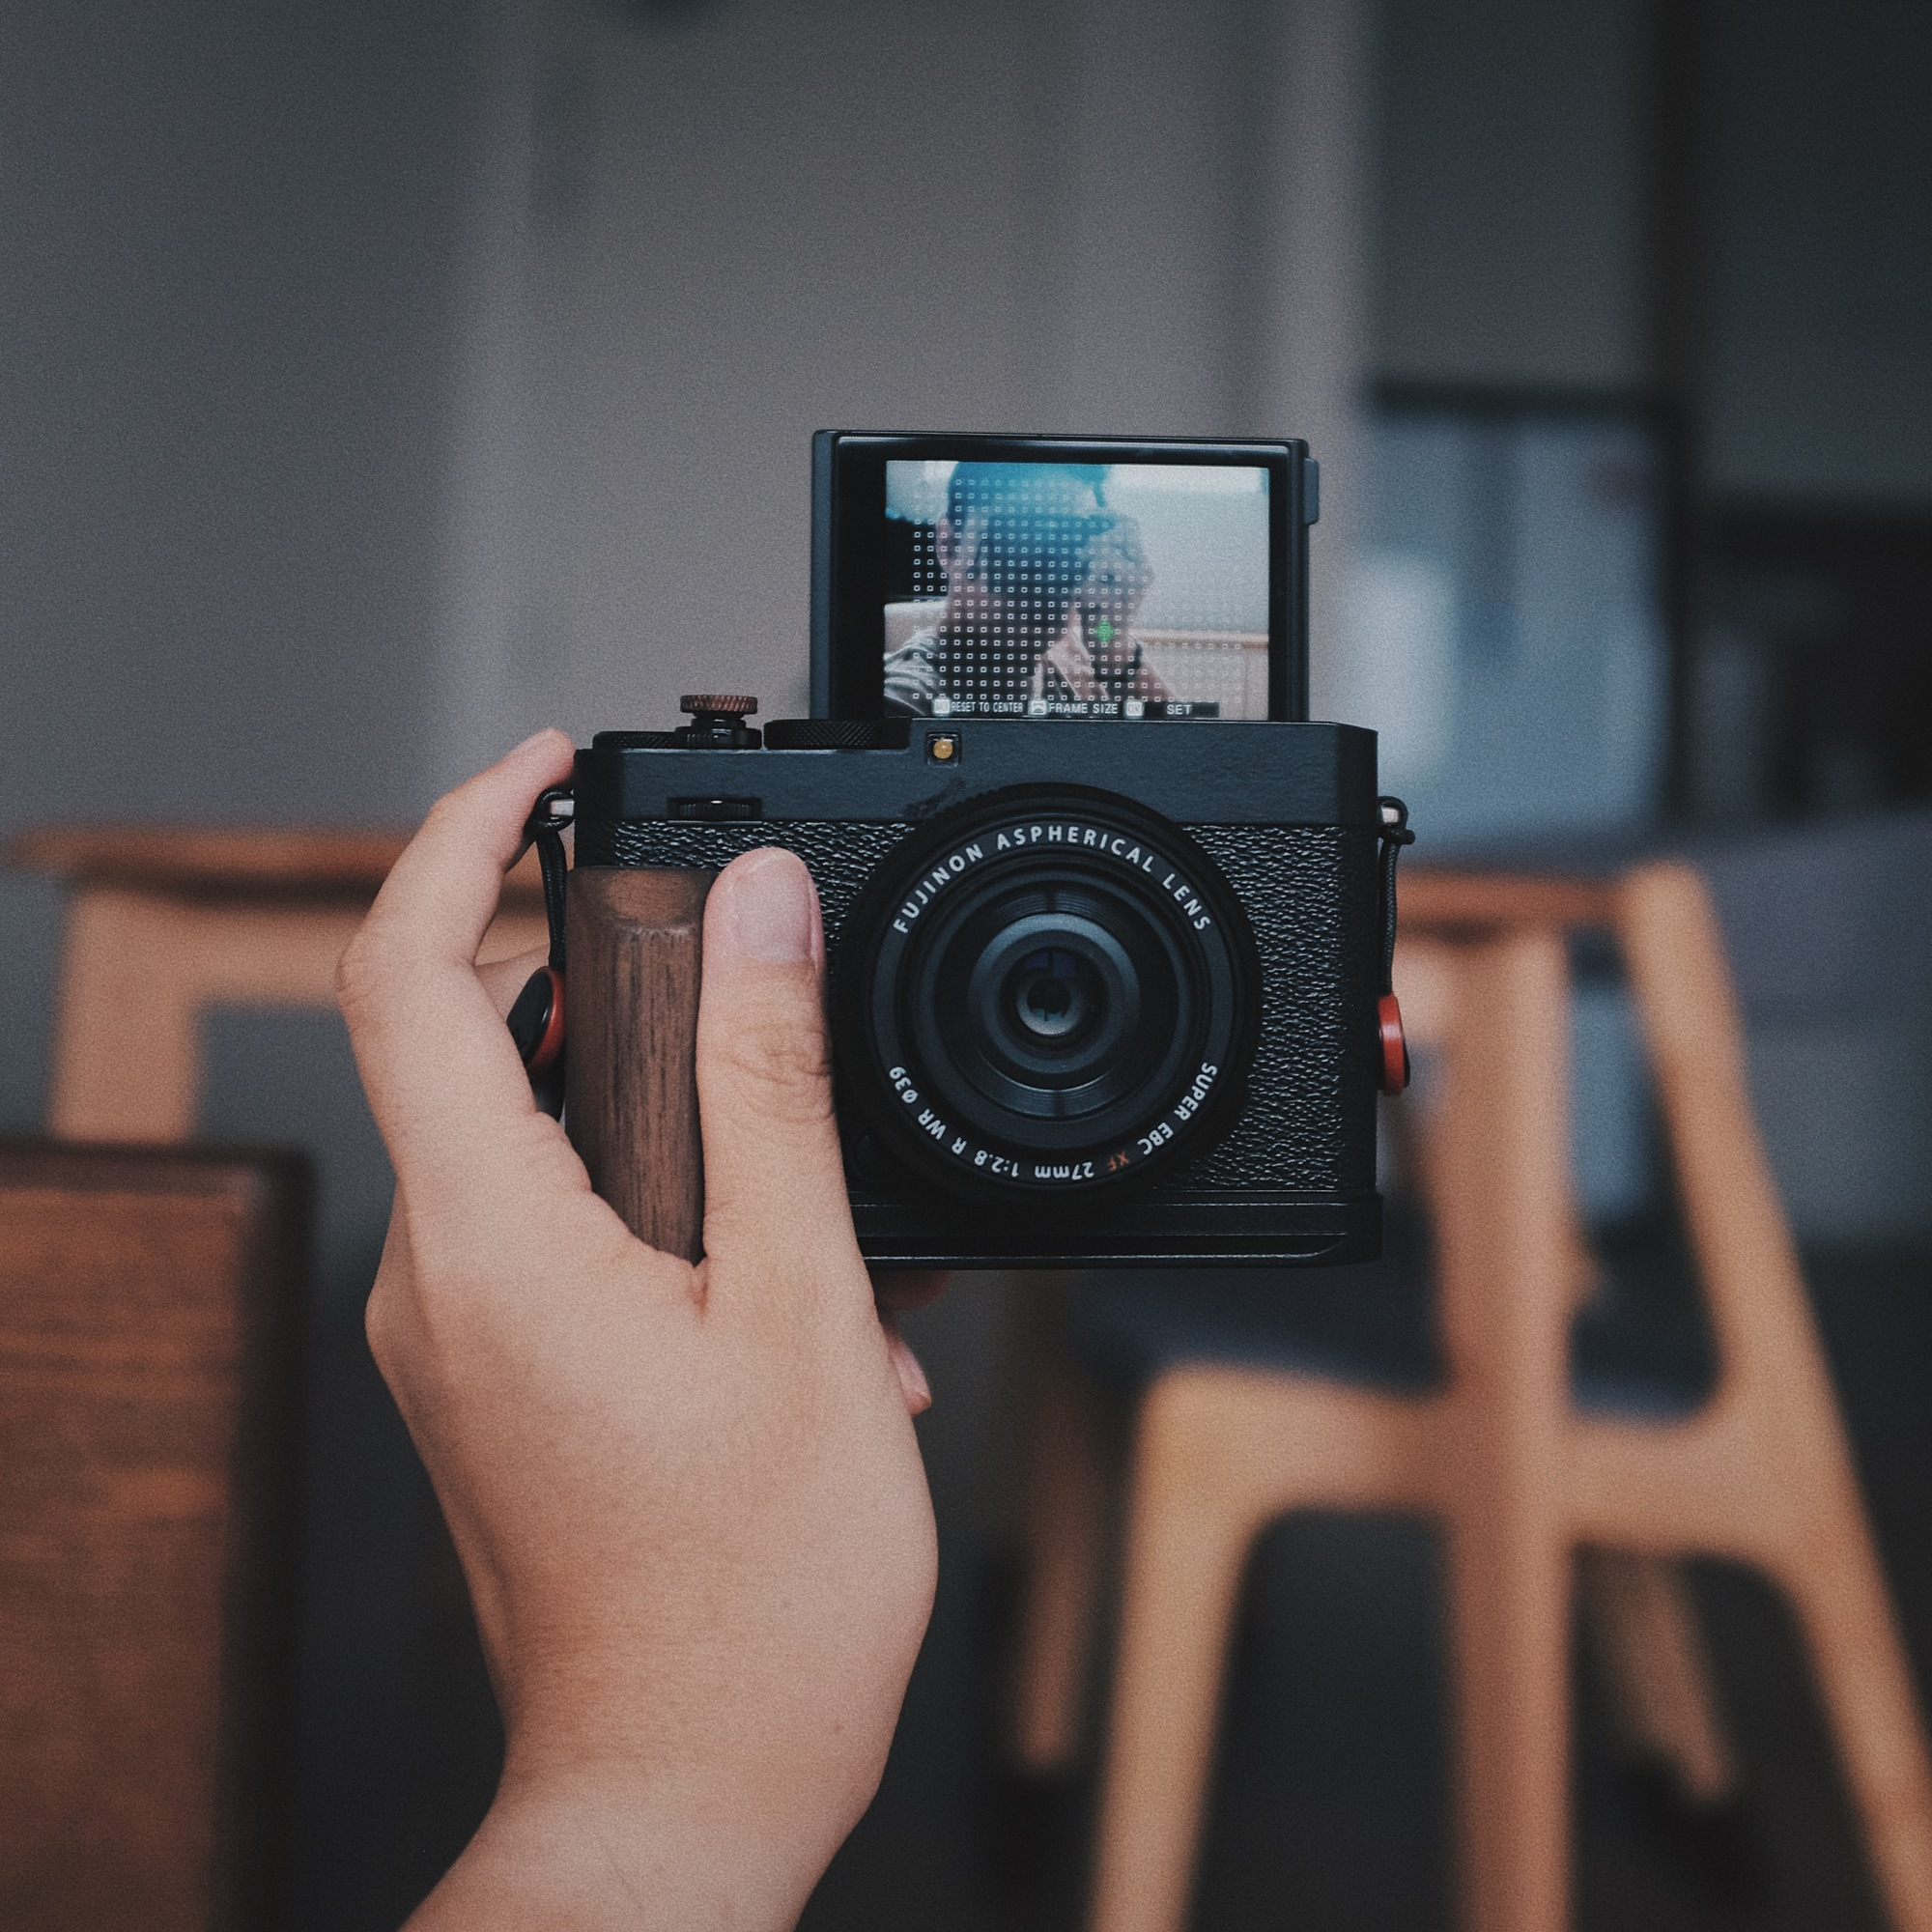
\includegraphics[width=\linewidth]{\envfinaldir/coverpic-prod.jpg}\par
            % \vskip 30pt
            \vfill

            \normalsize\rmfamily\scshape
            \copyright{} The Web Digest Project \hfill\large \envdatestr
        \end{center}
    \end{titlepage}
    % \restoregeometry
}
\newcommand{\simplehref}[1]{%
    \textcolor{blue!80!green}{\href{#1}{#1}}%
}
\renewcommand{\contentsname}{\center\Huge\sffamily\bfseries Contents\par\vskip 20pt}
\newcounter{ipartcounter}
\setcounter{ipartcounter}{0}
\newcommand{\ipart}[1]{
    % \vskip 20pt
    \clearpage
    \stepcounter{ipartcounter}
    \phantomsection
    \addcontentsline{toc}{chapter}{#1}
    % \begin{center}
    %     \Huge
    %     \sffamily\bfseries
    %     #1
    % \end{center}
    % \vskip 20pt plus 7pt
}
\newcounter{ichaptercounter}
\setcounter{ichaptercounter}{0}
\newcommand{\ichapter}[1]{
    % \vskip 20pt
    \clearpage
    \stepcounter{ichaptercounter}
    \phantomsection
    \addcontentsline{toc}{section}{\numberline{\arabic{ichaptercounter}}#1}
    \begin{center}
        \Huge
        \sffamily\bfseries
        #1
    \end{center}
    \vskip 20pt plus 7pt
}
\newcommand{\entrytitlefont}[1]{\subsection*{\raggedright\Large\sffamily\bfseries#1}}
\newcommand{\entryitemGeneric}[2]{
    % argv: title, url
    \parbox{\linewidth}{
        \entrytitlefont{#1}\par\vskip 5pt
        \footnotesize\ttfamily\mdseries
        \simplehref{#2}
    }\vskip 11pt plus 11pt minus 1pt
}
\newcommand{\entryitemGithub}[3]{
    % argv: title, url, desc
    \parbox{\linewidth}{
        \entrytitlefont{#1}\par\vskip 5pt
        \footnotesize\ttfamily\mdseries
        \simplehref{#2}\par\vskip 5pt
        \small\rmfamily\mdseries#3
    }\vskip 11pt plus 11pt minus 1pt
}
\newcommand{\entryitemAp}[3]{
    % argv: title, url, desc
    \parbox{\linewidth}{
        \entrytitlefont{#1}\par\vskip 5pt
        \footnotesize\ttfamily\mdseries
        \simplehref{#2}\par\vskip 5pt
        \small\rmfamily\mdseries#3
    }\vskip 11pt plus 11pt minus 1pt
}
\newcommand{\entryitemHackernews}[3]{
    % argv: title, hnurl, rawurl
    % \parbox{\linewidth}{
    %     \entrytitlefont{#1}\par\vskip 5pt
    %     \footnotesize\ttfamily\mdseries
    %     \simplehref{#3}\par
    %     \textcolor{black!50}{\href{#2}{#2}}
    % }\vskip 11pt plus 11pt minus 1pt
    \begin{minipage}{\linewidth}
            \entrytitlefont{#1}\par\vskip 5pt
            \footnotesize\ttfamily\mdseries
            \simplehref{#3}\par
            \textcolor{black!50}{\href{#2}{#2}}
    \end{minipage}\par\vskip 11pt plus 11pt minus 1pt
}







\begin{document}

\makeheader

\tableofcontents\clearpage




\ipart{Developers}
\ichapter{Hacker News}
\entryitemTwoLinks{New sphere-packing record stems from an unexpected source}{https://news.ycombinator.com/item?id=44493196}{https://www.quantamagazine.org/new-sphere-packing-record-stems-from-an-unexpected-source-20250707/}

\entryitemTwoLinks{My first verified imperative program}{https://news.ycombinator.com/item?id=44492986}{https://markushimmel.de/blog/my-first-verified-imperative-program/}

\entryitemTwoLinks{Adding a feature because ChatGPT incorrectly thinks it exists}{https://news.ycombinator.com/item?id=44491071}{https://www.holovaty.com/writing/chatgpt-fake-feature/}

\entryitemTwoLinks{Launch HN: Morph (YC S23) – Apply AI code edits at 4,500 tokens/sec}{https://news.ycombinator.com/item?id=44490863}{https://news.ycombinator.com/item?id=44490863}

\entryitemTwoLinks{Show HN: NYC Subway Simulator and Route Designer}{https://news.ycombinator.com/item?id=44490588}{https://buildmytransit.nyc}

\entryitemTwoLinks{CPU-X: CPU-Z for Linux}{https://news.ycombinator.com/item?id=44490386}{https://thetumultuousunicornofdarkness.github.io/CPU-X/}

\entryitemTwoLinks{I used o3 to profile myself from my saved Pocket links}{https://news.ycombinator.com/item?id=44489803}{https://noperator.dev/posts/o3-pocket-profile/}

\entryitemTwoLinks{Mercury: Ultra-fast language models based on diffusion}{https://news.ycombinator.com/item?id=44489690}{https://arxiv.org/abs/2506.17298}

\entryitemTwoLinks{Ask HN: Any resources for finding non-smart appliances?}{https://news.ycombinator.com/item?id=44488810}{https://news.ycombinator.com/item?id=44488810}

\entryitemTwoLinks{Anthropic cut up millions of used books, and downloaded 7M pirated ones – judge}{https://news.ycombinator.com/item?id=44488331}{https://www.businessinsider.com/anthropic-cut-pirated-millions-used-books-train-claude-copyright-2025-6}

\entryitemTwoLinks{Deno 2.4}{https://news.ycombinator.com/item?id=44488107}{https://deno.com/blog/v2.4}

\entryitemTwoLinks{Bitchat – A decentralized messaging app that works over Bluetooth mesh networks}{https://news.ycombinator.com/item?id=44485342}{https://github.com/jackjackbits/bitchat}

\entryitemTwoLinks{Swedish Campground (2004)}{https://news.ycombinator.com/item?id=44485241}{https://www.folklore.org/Swedish\_Campground.html}

\entryitemTwoLinks{The Broken Microsoft Pact: Layoffs and Performance Management}{https://news.ycombinator.com/item?id=44484874}{https://danielsada.tech/blog/microsoft-pact/}

\entryitemTwoLinks{Intel's Lion Cove P-Core and Gaming Workloads}{https://news.ycombinator.com/item?id=44484688}{https://chipsandcheese.com/p/intels-lion-cove-p-core-and-gaming}

\entryitemTwoLinks{A non-anthropomorphized view of LLMs}{https://news.ycombinator.com/item?id=44484682}{http://addxorrol.blogspot.com/2025/07/a-non-anthropomorphized-view-of-llms.html}

\entryitemTwoLinks{Nobody has a personality anymore: we are products with labels}{https://news.ycombinator.com/item?id=44484595}{https://www.freyaindia.co.uk/p/nobody-has-a-personality-anymore}

\entryitemTwoLinks{Building the Rust Compiler with GCC}{https://news.ycombinator.com/item?id=44484363}{https://fractalfir.github.io/generated\_html/cg\_gcc\_bootstrap.html}

\entryitemTwoLinks{LLMs should not replace therapists}{https://news.ycombinator.com/item?id=44484207}{https://arxiv.org/abs/2504.18412}

\entryitemTwoLinks{Why English doesn't use accents}{https://news.ycombinator.com/item?id=44484137}{https://www.deadlanguagesociety.com/p/why-english-doesnt-use-accents}


\ipart{Developers~~~~(zh-Hans)}
\ichapter{Solidot}
\entryitemGeneric{\hskip 0pt{}三星手机电池次数显著高于其它品牌}{https://www.solidot.org/story?sid=81740}

\entryitemGeneric{\hskip 0pt{}印度关闭互联网的次数高居第一}{https://www.solidot.org/story?sid=81739}

\entryitemGeneric{\hskip 0pt{}为什么杀人鲸朝我们扔鱼}{https://www.solidot.org/story?sid=81738}

\entryitemGeneric{\hskip 0pt{}Moderna 称 mRNA 流感疫苗有效性高于标准疫苗}{https://www.solidot.org/story?sid=81737}

\entryitemGeneric{\hskip 0pt{}美元正经历现代史上最糟糕的一年}{https://www.solidot.org/story?sid=81736}

\entryitemGeneric{\hskip 0pt{}企业已经感受到气候变暖的影响}{https://www.solidot.org/story?sid=81735}

\entryitemGeneric{\hskip 0pt{}经历双重引爆的超新星}{https://www.solidot.org/story?sid=81734}

\entryitemGeneric{\hskip 0pt{}StatCounter 统计显示 Windows 11 的市场份额超过了 Windows 10}{https://www.solidot.org/story?sid=81733}

\entryitemGeneric{\hskip 0pt{}Valve 征服了 PC 游戏}{https://www.solidot.org/story?sid=81732}

\entryitemGeneric{\hskip 0pt{}微软关闭巴基斯坦业务}{https://www.solidot.org/story?sid=81731}

\entryitemGeneric{\hskip 0pt{}研究称加工肉没有食用的安全量}{https://www.solidot.org/story?sid=81730}

\entryitemGeneric{\hskip 0pt{}微软 XBox 业务高管建议被裁员的员工用 AI 管理情绪}{https://www.solidot.org/story?sid=81729}\ichapter{V2EX}
\entryitemGeneric{\hskip 0pt{}[C++] 想系统的学习 Modern C++,麻烦大佬们推荐一些书籍}{https://www.v2ex.com/t/1143633}

\entryitemGeneric{\hskip 0pt{}[Apple] Apple ID 换区对 Developer Program 有影响吗}{https://www.v2ex.com/t/1143632}

\entryitemGeneric{\hskip 0pt{}[加密货币] \$v2ex 都买了吗?}{https://www.v2ex.com/t/1143631}

\entryitemGeneric{\hskip 0pt{}[VXNA] 申请收录站点 https://1900.live}{https://www.v2ex.com/t/1143629}

\entryitemGeneric{\hskip 0pt{}[问与答] 新系统做大数据解析是否需要上 hadoop}{https://www.v2ex.com/t/1143628}

\entryitemGeneric{\hskip 0pt{}[VXNA] 申请收录个人博客 blog.liuhao.im}{https://www.v2ex.com/t/1143627}

\entryitemGeneric{\hskip 0pt{}[酷工作] [南京/北京] AI start-up 招 react/vue/node 实习同学 300-500 元/天}{https://www.v2ex.com/t/1143623}

\entryitemGeneric{\hskip 0pt{}[Apple] macOS 26 beta3 更新完 眼前一亮的感觉}{https://www.v2ex.com/t/1143621}

\entryitemGeneric{\hskip 0pt{}[宽带症候群] 部分 Cloudflare 的域名近期在大陆无法访问}{https://www.v2ex.com/t/1143620}

\entryitemGeneric{\hskip 0pt{}[Apple] beta3 来啦, iOS26 已检测到,但 Tahoe 还没推送到。}{https://www.v2ex.com/t/1143619}

\entryitemGeneric{\hskip 0pt{}[职场话题] 第一次喜提副业,竟然不是兴奋,而是有点焦虑}{https://www.v2ex.com/t/1143616}

\entryitemGeneric{\hskip 0pt{}[问与答] win11 如何快速概览文件路径下的文件夹大小}{https://www.v2ex.com/t/1143615}

\entryitemGeneric{\hskip 0pt{}[问与答] 只有微信原始 ID(wxid\_XXXXXXXXX)怎么加好友}{https://www.v2ex.com/t/1143613}

\entryitemGeneric{\hskip 0pt{}[分享发现] 关键词工具}{https://www.v2ex.com/t/1143612}

\entryitemGeneric{\hskip 0pt{}[问与答] 好奇,为啥 windows 一登陆微信,手机微信列表的服务号都不显示了?}{https://www.v2ex.com/t/1143611}

\entryitemGeneric{\hskip 0pt{}[投资] 推荐个券商}{https://www.v2ex.com/t/1143610}

\entryitemGeneric{\hskip 0pt{}[问与答] 在知道部分密码的情况下,智能门锁的``虚位密码''功能会导致安全性下降多少?}{https://www.v2ex.com/t/1143608}

\entryitemGeneric{\hskip 0pt{}[宽带症候群] 家里联通公网 ip, wireguard 回家,移动网络回家速度比联通网络回家速度快,什么原因?}{https://www.v2ex.com/t/1143607}

\entryitemGeneric{\hskip 0pt{}[Edge] 招笑微软 Edge 浏览器默认新标签页直接报错}{https://www.v2ex.com/t/1143605}

\entryitemGeneric{\hskip 0pt{}[职场话题] 寒冬之下,一个双非 Java 仔的迷茫与破局之路}{https://www.v2ex.com/t/1143604}

\entryitemGeneric{\hskip 0pt{}[Apple] 明天是不是更新 beta3 了}{https://www.v2ex.com/t/1143603}

\entryitemGeneric{\hskip 0pt{}[职场话题] 公司开始利用 Ai 管理考核程序员的工作效率了}{https://www.v2ex.com/t/1143602}

\entryitemGeneric{\hskip 0pt{}[酷工作] [上海] Insomnia 团队招后台 Golang 开发}{https://www.v2ex.com/t/1143601}

\entryitemGeneric{\hskip 0pt{}[iPhone] 现在如何买外区的苹果礼品卡}{https://www.v2ex.com/t/1143600}

\entryitemGeneric{\hskip 0pt{}[分享发现] 同志们,我好像搞懂经济了,但是随之而来一个无法理解的事情……}{https://www.v2ex.com/t/1143598}

\entryitemGeneric{\hskip 0pt{}[职场话题] 做个小调查,大家公司有明确的晋升流程吗?有槽点吗?}{https://www.v2ex.com/t/1143597}

\entryitemGeneric{\hskip 0pt{}[分享创造] 分享一下我的新项目:智能域名搜索工具}{https://www.v2ex.com/t/1143595}

\entryitemGeneric{\hskip 0pt{}[职场话题] 北京望京的康明斯外包开发岗, xdm 有了解的吗}{https://www.v2ex.com/t/1143594}

\entryitemGeneric{\hskip 0pt{}[奇思妙想] 想做一个英语面试练习的智能体}{https://www.v2ex.com/t/1143592}

\entryitemGeneric{\hskip 0pt{}[English] 《大展鸿图》歌词:我说是对兄弟不是 pusy, pusy 粤语里有特殊含义?}{https://www.v2ex.com/t/1143588}

\entryitemGeneric{\hskip 0pt{}[分享创造] 上线了一个自动起卦 AI 解卦工具,支持大衍筮法、梅花易数,还有 64 卦供易经爱好者学习}{https://www.v2ex.com/t/1143587}

\entryitemGeneric{\hskip 0pt{}[问与答] Apple 的 Proton, Apple Game Porting Toolkit 现在怎么样了?}{https://www.v2ex.com/t/1143586}

\entryitemGeneric{\hskip 0pt{}[问与答] 兄弟们, 做 IT Infrastructure/基础设施的数据中心/Data Center,是不是竞争很小?}{https://www.v2ex.com/t/1143585}

\entryitemGeneric{\hskip 0pt{}[Cursor] 大家 cursor pro 都切回旧的 500 次计费方式了吗?}{https://www.v2ex.com/t/1143582}

\entryitemGeneric{\hskip 0pt{}[VPS] 1 元机场 30G}{https://www.v2ex.com/t/1143581}

\entryitemGeneric{\hskip 0pt{}[分享创造] 键盘风暴+AI:一个 idea 制造机 2}{https://www.v2ex.com/t/1143579}

\entryitemGeneric{\hskip 0pt{}[Linux] Linux mint 在低配笔记本上很好用}{https://www.v2ex.com/t/1143577}

\entryitemGeneric{\hskip 0pt{}[推广] [远程 web3 岗位推荐] 现在有 30+的 web3 远程岗位,给各位内推一下}{https://www.v2ex.com/t/1143576}

\entryitemGeneric{\hskip 0pt{}[生活] 媳妇事业节节高,我感觉自己快成``拖后腿''的了}{https://www.v2ex.com/t/1143572}

\entryitemGeneric{\hskip 0pt{}[酷工作] Avenir Group 测试、大前端、平台产品职位}{https://www.v2ex.com/t/1143571}

\entryitemGeneric{\hskip 0pt{}[成都] 想购车但是不清楚成都得各项补贴情况,求科普}{https://www.v2ex.com/t/1143570}

\entryitemGeneric{\hskip 0pt{}[旅行] 想跟女友暑假去西部玩一趟,有什么推荐吗?}{https://www.v2ex.com/t/1143569}

\entryitemGeneric{\hskip 0pt{}[问与答] 有没有经常跑高速的电车车友?高速买啥电卡划算}{https://www.v2ex.com/t/1143568}

\entryitemGeneric{\hskip 0pt{}[深圳] 深圳宝安福永福海求租个两房, 有什么好推荐?}{https://www.v2ex.com/t/1143567}

\entryitemGeneric{\hskip 0pt{}[问与答] Toyota Super A90 下位替代}{https://www.v2ex.com/t/1143566}

\entryitemGeneric{\hskip 0pt{}[远程工作] [远程] Java 开发工程师 (3-5 位)}{https://www.v2ex.com/t/1143565}

\entryitemGeneric{\hskip 0pt{}[问与答] 有没有瘦子增重成功的过来人指点下我}{https://www.v2ex.com/t/1143564}

\entryitemGeneric{\hskip 0pt{}[科技] 手游自动化脚本}{https://www.v2ex.com/t/1143563}

\entryitemGeneric{\hskip 0pt{}[OpenAI] Claude Code 或者 Gemini 真的比 Cursor 好用吗?}{https://www.v2ex.com/t/1143562}

\entryitemGeneric{\hskip 0pt{}[职场话题] 小弟运维,有跳槽的想法了,想请教下各位的意见}{https://www.v2ex.com/t/1143561}


\ipart{Generic News}







\clearpage
\leavevmode\vfill
\footnotesize

Copyright \copyright{} 2023-2025 Neruthes and other contributors.

This document is published with CC BY-NC-ND 4.0 license.

The entries listed in this newsletter may be copyrighted by their respective creators.

This newsletter is generated by the Web Digest project.

The newsletters are also delivered via Telegram channel \CJKunderline{\href{https://t.me/webdigestchannel}{https://t.me/webdigestchannel}}.\\
RSS feed is available at \CJKunderline{\href{https://webdigest.pages.dev/rss.xml}{https://webdigest.pages.dev/rss.xml}}.

This newsletter is available in PDF at
\CJKunderline{\href{https://webdigest.pages.dev/}{https://webdigest.pages.dev/}}.

The source code being used to generate this newsletter is available at\\
\CJKunderline{\href{https://github.com/neruthes/webdigest}{https://github.com/neruthes/webdigest}}.

This newsletter is also available in
\CJKunderline{\href{http://webdigest.pages.dev/readhtml/\envyear/WebDigest-20250708.html}{HTML}} and
\CJKunderline{\href{https://github.com/neruthes/webdigest/blob/master/markdown/\envyear/WebDigest-20250708.md}{Markdown}}.


\coverpic{https://unsplash.com/photos/foggy-mountain-peak-amidst-the-clouds-NofNB4LNz7Q}{Jonas Degener}


\end{document}
